\chapter{Probabilistic modeling of team dynamics}
\label{ch:pgm}
\textbf{Paulo Soares, Kobus Barnard, Emily Butler}
\section{Introduction}
\begin{itemize}
    \item Why is this a useful capability for an AI
        agent? How does it contribute to machine theory of mind/machine theory
        of teams?
    \item What are the existing state of the art approaches to this problem
        (cite relevant papers), and what are their limitations? 
    \item What is our approach, and how will it address those limitations?
\end{itemize}

\section{Approach}

Our agent is comprised of a \emph{cognitive} and a \emph{memory} module. The agent uses the cognitive module to reason about the participant minds probabilistically. The quality of a team is explicitly represented in the architecture as a latent random variable and it is closely related to the score of the team. The team quality is directly affected by how coordinated the team is. A visual representation of the cognitive module is illustrated in Figure \ref{fig:pgm}. 

\begin{figure}[htb]
\centering
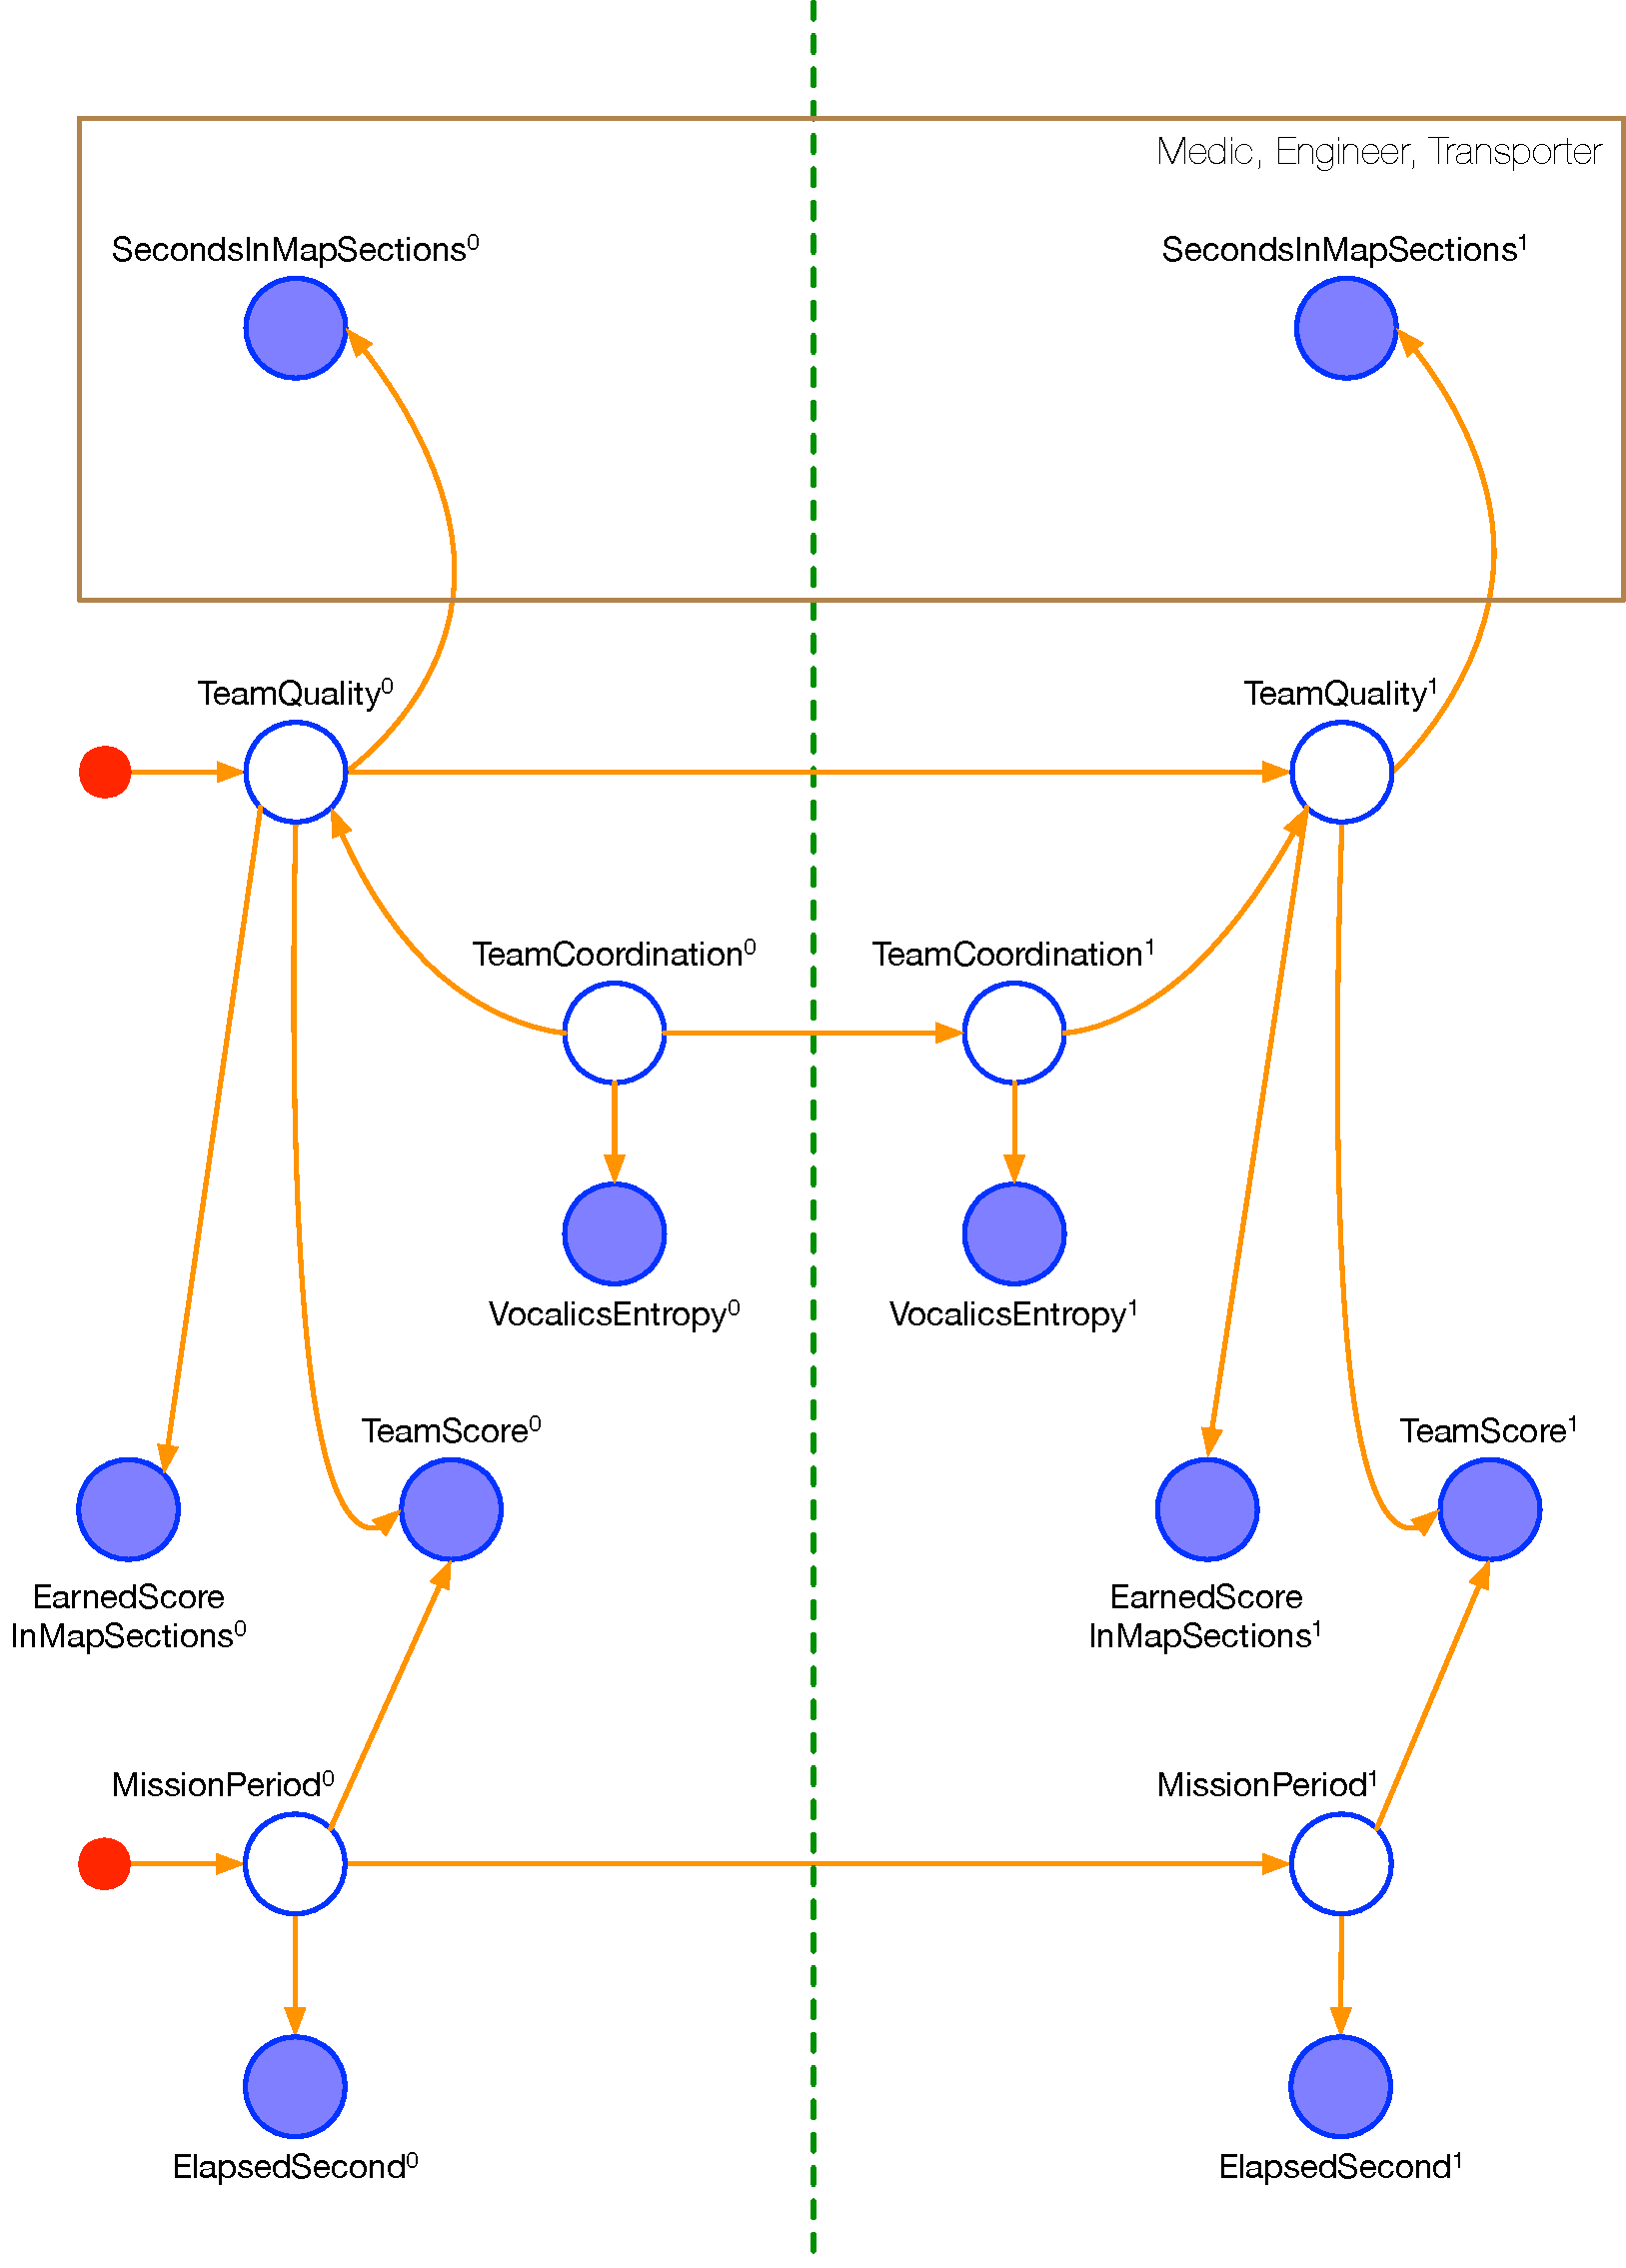
\includegraphics[width=\textwidth]{images/pgm}	
\caption{Cognitive module represented as a dynamic Bayes network. For simplicity, only the two first time steps are represented in the image. The model encodes the assumption that different levels of coordination among teammates directly affect the team quality. Moreover, the team quality is closely related to the score earned by the team and amount of time spent in different areas of the map.}
\label{fig:pgm}
\end{figure}

For intervention purposes, the agent also possesses a memory module to keep track of relevant information that will later be given/reminded to the participants. The agent will decide the right moment to communicate with the team, based on inferences and predictions of the team quality. For instance, to decide whether participants should stop their current task to go help another teammate to wake up a critical victim, the agent might estimate the amount of time taken for the participants to get where the critical victim is, and check if the score earned with the critical victim is superior to the score potentially earned if the participants continue to perform their current tasks. 

The list of variables used as evidence for both modules is presented in Table \ref{tab:pgm_evidence_list}. 

\begin{table*}[tb]
\centering
\begin{tabular}{ll}
    \toprule
    Variable & Description \\\midrule
    MinecraftEntity\_Event\_Scoreboard\_Simulator & Used to determine the current score of the team. \\
    MinecraftEntity\_Event\_Triage\_Simulator & Used to compute how many points were earned in different parts of the map. \\
    MinecraftEntity\_Event\_Proximityvictiminteraction\_Simulator & Used to remove a victim from the list of unstabilized critical victims previously observed. \\
    MinecraftEntity\_Event\_Playerfrozenstatechange\_Simulator & Used to keep track of trapped participants. \\
    MinecraftEntity\_Event\_Markerplaced\_Simulator & Used to keep track of threat room and victim identification. \\
    MinecraftEntity\_Event\_Markerremoved\_Simulator & Used to keep track of threat room and victim identification. \\
    MinecraftEntity\_Event\_Markerdestroyed\_Simulator & Used to keep track of threat room and victim identification. \\
    MinecraftEntity\_Event\_Victimpickedup\_Simulator & Used to determine whether to inform the participant about the victim type or not. \\
    MinecraftEntity\_Event\_Victimplaced\_Simulator & Used to determine whether the victim was placed in an incorrect safe zone. \\
    MinecraftEntity\_Event\_Rubbledestroyed\_Simulator & Used to reassess whether any previously observed trapped victims became reachable. \\   
    MinecraftEntity\_Event\_Missionstate\_Simulator & Used to identify the beginning and end of a mission. \\
    MinecraftEntity\_Trial\_Startstop\_Testbedcontroller & Used to collect information about the players and identify the mission map. \\
    MinecraftEntity\_Observation\_Fov\_Fovtool & Used to determine trapped victims that were observed by the participants. \\
    MinecraftEntity\_Observation\_State\_Simulator & Used to determine the location of the participants in the map. \\
    Audio & Used to extract vocalic features from the communication among the participants. \\
    \bottomrule
\end{tabular}
\caption{List of variables used as evidence by the agent.}
\label{tab:pgm_evidence_list}
\end{table*}

\subsection{Interventions}

By reasoning about what the participants are doing, an agent can provide valuable information to instill them to adopt better strategies, encourage them whenever they are doing a good work and remind them about important events they might have forgotten. 
            
Therefore, the objective of our agent is to improve the final team score by reasoning about the quality of the team and acting to avoid its degradation throughout the mission. To accomplish that objective, our agent is equipped with the following list of interventions

\subsubsection{Global Interventions}

\begin{description}
    \item[\textbf{Team Quality:}] based on the current agent's belief about the team quality, the agent informs the teammates about their performance so far.
        
    \emph{Rationale}: Participants might not have a notion of how well they are performing until they have been told, especially in early stages of the mission. Knowing about their performance compared to other teams is likely to encourage weak teams to change their strategy to achieve better performance. 
    
    \item[\textbf{Stabilization Postponement:}] when a critical victim is spotted by the medic, the agent estimates how long it would take the closest player to arrive at the victim location. If it’s spotted by another specialist, the agent estimates how long it would take the medic to arrive at the location. In case it takes a large amount of time, the agent suggests to the team to mark the victim, move on and hold that rescue for a while. The agent keeps track of marked victims to alert players at appropriate times in the future. 
        
    \emph{Rationale}: If it takes a lot of time to rescue a single critical victim, it is more reasonable that the participants do not get distracted from their current tasks, and focus on saving the critical victims later when they are doing other tasks nearby.
   
    \item[\textbf{Remaining Time:}] the agent alerts the team about how many minutes they have left until the end of the mission.
        
    \emph{Rationale}: The team might not be paying attention to the timer. Reminding them about the time they have left might encourage them to switch to a better strategy close to the end of the mission. For instance, move all pending victims to the safe zones.
    
    \item[\textbf{Team Coordination:}] based on the entropy of the vocalic features of the participants, the agent infers how coordinated the team is and lets them know as soon as the level drops below a certain threshold.  
        
    \emph{Rationale}: When people talk to each other cooperatively, they begin to exhibit 'entrainment', in which physical, gestural and speech behaviors begin to align more closely. In phonetic aspects of speech, entrainment can appear in, for example, speech rate, loudness, voice quality, vowel production, intonation, and many other dimensions of variation. Conversely, when interlocutors are not cooperative or have a negative attitude toward their interaction, they can fail to entrain or even exhibit 'disentrainment', in which their speech patterns become more distinct. Turning this around, analyzing measures of entrainment between interlocutors can help us predict whether they are successfully cooperating and whether they have a positive attitude toward each other.
\end{description}
    
\subsubsection{Targeted Interventions}

\begin{description}
    \item[\textbf{Exploration Diversity:}] based on the amount of time a given participant has spent in a specific section of the map, the agent suggests the participant to explore a different part of the map if keeping exploring the current area longer is likely to degrade the team’s quality.
        
    \emph{Rationale}: There’s an optimal expected amount of time that each specialist is supposed to spend in different parts of the map. E.g. After clearing rubles in a certain area, the engineer should move to other parts of the map; going back to cleared areas sporadically for tasks that require team cooperation. If the amount of time spent in a certain area is too far from that expected optimum, it is expected that most of the required tasks for that area have already been completed and the participant should move to a different part of the map.
    
    \item[\textbf{Victim Reachability:}] the agent keeps track of all unreachable victims spotted by the medic and updates their status whenever the engineer clears the path towards them. The agent uses that information to inform the medic whenever they are nearby now reachable victims but deviate from rescuing them.
        
    \emph{Rationale}: The medic is likely to not remember all the victims seen along the way, even less their current reachability status. If the agent believes the medic does not know about their proximity to a reachable victim, it must inform the medic right away so the victim can be rescued.
    
    \item[\textbf{Threat Room Identification:}] the agent reminds engineers to place markers in the threat rooms in case they have forgotten to do so.
        
    \emph{Rationale}: Only the engineer knows about threat rooms in the beginning. If the engineer passes or enters such a room and does not mark it as a threat, the agent must remind the participant to do so to reduce the chance that others get trapped unnecessarily.

	\item[\textbf{Victim Identification:}] the agent reminds the medic to place the correct marker nearby a stabilized victim if no marker has been placed. Even so, the agent will keep track of non-marked victims to let whoever is transporting the victim know about its correct type.
        
    \emph{Rationale}: If the medic does not identify the victim right before or after stabilization, the participants will not be able to tell which type of injury that victim has and will not be able to move it to the correct safe zone later.
    
    \item[\textbf{Critical Victim Proximity:}] this intervention is a result of the stabilization postponement global intervention. When the agent detects that the medic and another participant are close enough to an unstabilized previously spotted critical victim, it reminds those participants about that victim's existence.
        
    \emph{Rationale}: See Stabilization Postponement global intervention.    
    
    \item[\textbf{Rescue Postponement:}] when a participant other than the engineer gets trapped in a room, let the engineer knows whether to rescue the other participant right away or whether it can wait for a while. 
        
    \emph{Rationale}: If the task the engineer is currently doing is more likely to improve the team score than going in rescue of another team member, the agent must let the engineer know about that.

\end{description}
 


%\begin{itemize}
%
%    \item Provide details on our approach, including:
%        \begin{itemize}
%            \item What data is required for this work? If any of the required
%                inputs are present in the table of Study 3 variables in the
%                \href{https://docs.google.com/document/d/1GF7VsNF9R95IAaj6mVZUDV2mAX5ok1Bh6Tcm8zDpIkg/edit#heading=h.1ksv4uv}{TA3
%                Study 3 preregistration document (table 3)}, please list those
%                variables with the standardized verbose variable names in the table.
%            \item What interventions will we be testing and why?
%        \end{itemize}
%\end{itemize}

\section{Evaluation}
\begin{itemize}
    \item How will we evaluate our approach?
\end{itemize}

